\documentclass[aspectratio=169,11pt]{beamer}

\usetheme{Madrid}
\usecolortheme{default}
\setbeamertemplate{navigation symbols}{}
\setbeamertemplate{caption}[numbered]

\usepackage[utf8]{inputenc}
\usepackage[T1]{fontenc}
\usepackage{graphicx}
\usepackage{booktabs}
\usepackage{amsmath}
\usepackage{xcolor}
\usepackage{array}
\usepackage{hyperref}

\graphicspath{{figures/}}

\definecolor{projectTeal}{HTML}{008C7A}
\definecolor{projectDark}{HTML}{1E1E1E}
\definecolor{projectMagenta}{HTML}{D000D0}
\definecolor{projectYellow}{HTML}{E6E600}

\setbeamercolor{title}{fg=white,bg=projectTeal}
\setbeamercolor{frametitle}{fg=white,bg=projectTeal}
\setbeamercolor{structure}{fg=projectTeal}
\setbeamercolor{block title}{fg=white,bg=projectTeal}
\setbeamercolor{block body}{fg=black,bg=projectTeal!6}
\setbeamertemplate{footline}
{
    \leavevmode
    \hbox{
        % Left: University
        \begin{beamercolorbox}[
            wd=.30\paperwidth,
            ht=2.5ex,
            dp=1ex,
            center
        ]{author in head/foot}
            \insertauthor
        \end{beamercolorbox}

        % Center: Title
        \begin{beamercolorbox}[
            wd=.40\paperwidth,
            ht=2.5ex,
            dp=1ex,
            center
        ]{title in head/foot}
            \insertshorttitle
        \end{beamercolorbox}

        % Right: Date + Slide Number
        \begin{beamercolorbox}[
            wd=.30\paperwidth,
            ht=2.5ex,
            dp=1ex,
            center
        ]{date in head/foot}
            \insertshortdate\hfill\insertframenumber/\inserttotalframenumber
        \end{beamercolorbox}
    }
    \vskip0pt
}
\title[Road Pitch Estimation in CARLA]{Road Pitch Estimation and Sensor Fusion in CARLA}
\subtitle{Semantic Camera Measurements, MobileNet Regression, and Kalman Filtering}
\author{R\"uzgar Bat\i{} Okay \& Alperen Tufan Pelit}
\institute{
Department of Electrical and Electronics Engineering\\
Marmara University
}
\date{EE4084 Project Video}

\newcommand{\smallnote}[1]{\vspace{0.35em}{\parbox{\linewidth}{\footnotesize\color{gray!80!black}#1}}}

\begin{document}

% ------------------------------------------------------------
\begin{frame}
    \titlepage
\end{frame}

% ------------------------------------------------------------
\begin{frame}{Video Roadmap}
\begin{columns}[T,onlytextwidth]
\column{0.48\textwidth}
\begin{block}{Main project explanation}
\begin{tabular}{@{}ll@{}}
0:00 & Introduction \\
0:20 & Contents \\
0:45 & Project goal \\
1:15 & Final system overview \\
2:00 & Results and discussion \\
\end{tabular}
\end{block}

\column{0.48\textwidth}
\begin{block}{Reproducibility and implementation}
\begin{tabular}{@{}ll@{}}
4:30 & Tools used \\
5:30 & Methods and theory \\
7:00 & Code structure \\
8:15 & Setup and running \\
9:30 & Conclusion \\
\end{tabular}
\end{block}
\end{columns}
\smallnote{The first part gives the project result and interpretation. Later sections explain how it was built and how it can be reproduced.}
\end{frame}

% ------------------------------------------------------------
\begin{frame}{Project Goal}
\begin{columns}[T,onlytextwidth]
\column{0.55\textwidth}
\begin{block}{Problem}
Road pitch affects vehicle longitudinal dynamics and autonomous driving state estimation.
\end{block}

\begin{block}{Goal}
Estimate road pitch in CARLA using multiple simulated sensing sources and compare the results with CARLA reference signals.
\end{block}

\column{0.40\textwidth}
\begin{block}{Signals used}
\begin{itemize}
    \item Semantic camera
    \item IMU gyroscope
    \item GNSS baseline
    \item CARLA vehicle pitch
    \item CARLA waypoint pitch
\end{itemize}
\end{block}
\end{columns}
\end{frame}

% ------------------------------------------------------------
\begin{frame}{Final Result First: Kalman Filter Output}
\begin{columns}[T,onlytextwidth]
\column{0.66\textwidth}
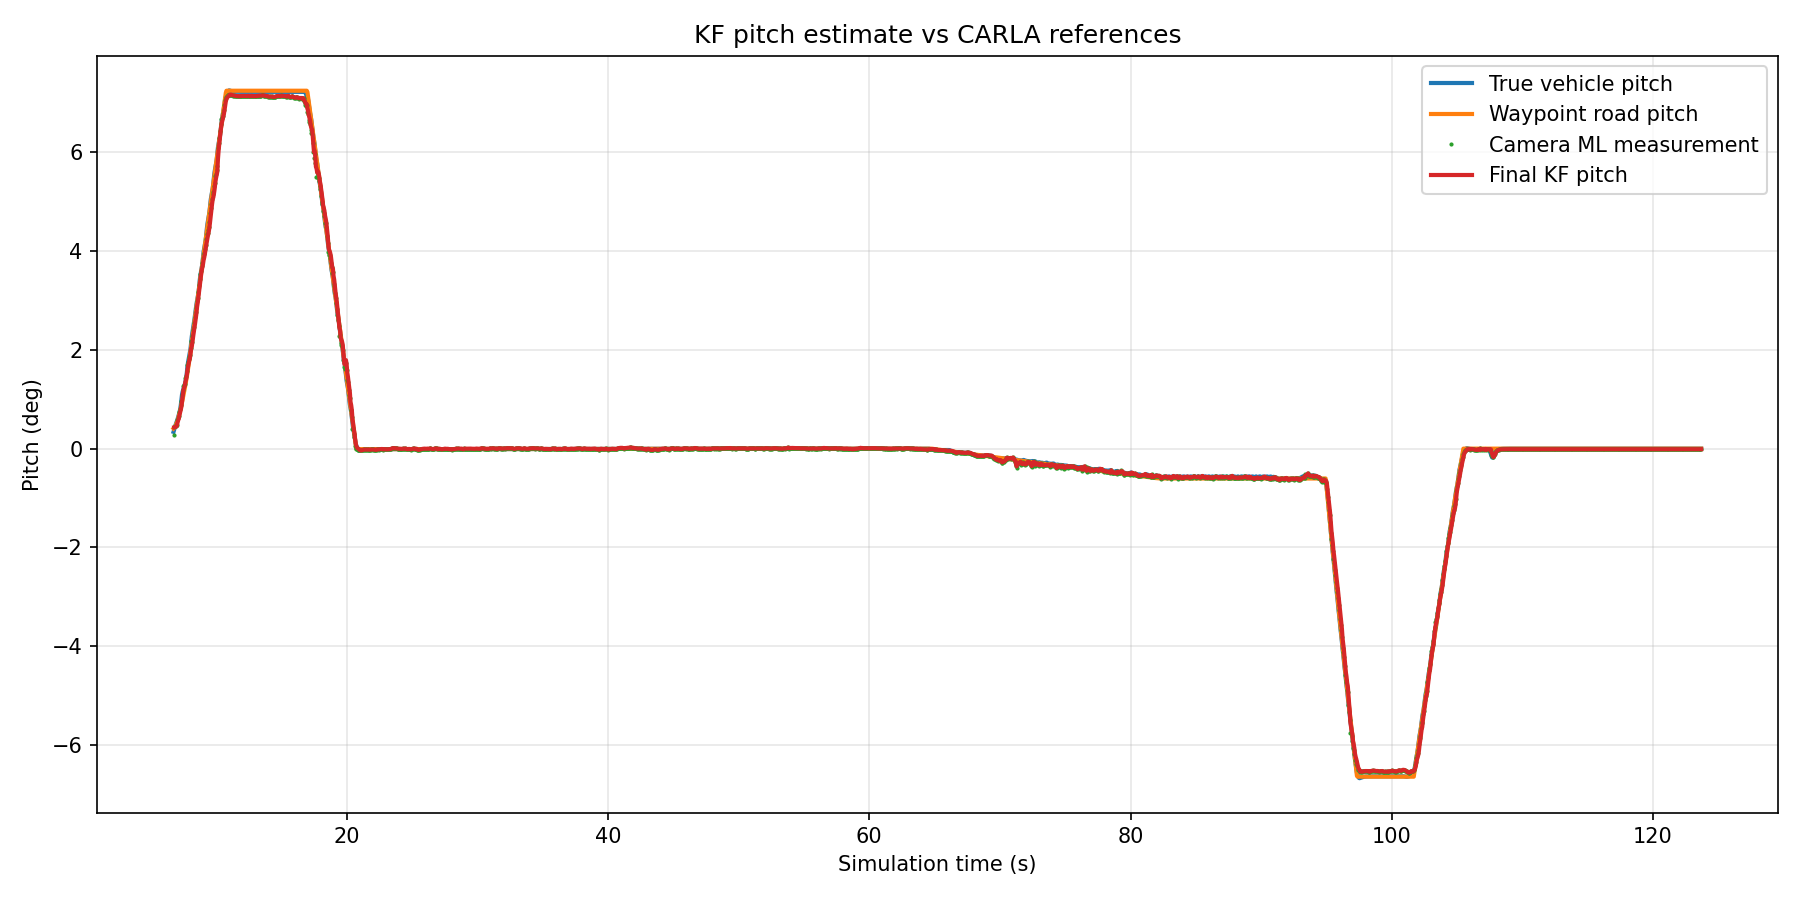
\includegraphics[width=\linewidth]{kf_pitch.png}
\column{0.31\textwidth}
\begin{block}{Main observation}
The Kalman Filter output follows the CARLA reference pitch closely during both uphill and downhill sections.
\end{block}
\begin{block}{Error summary}
\begin{tabular}{@{}lcc@{}}
\toprule
Estimate & MAE & RMSE \\
\midrule
Camera & 0.028$^\circ$ & 0.050$^\circ$ \\
KF & 0.034$^\circ$ & 0.063$^\circ$ \\
GNSS & 0.023$^\circ$ & 0.158$^\circ$ \\
\bottomrule
\end{tabular}
\end{block}
\end{columns}
\end{frame}

% ------------------------------------------------------------
\begin{frame}{What the Camera Model Sees}
\begin{columns}[T,onlytextwidth]
\column{0.62\textwidth}
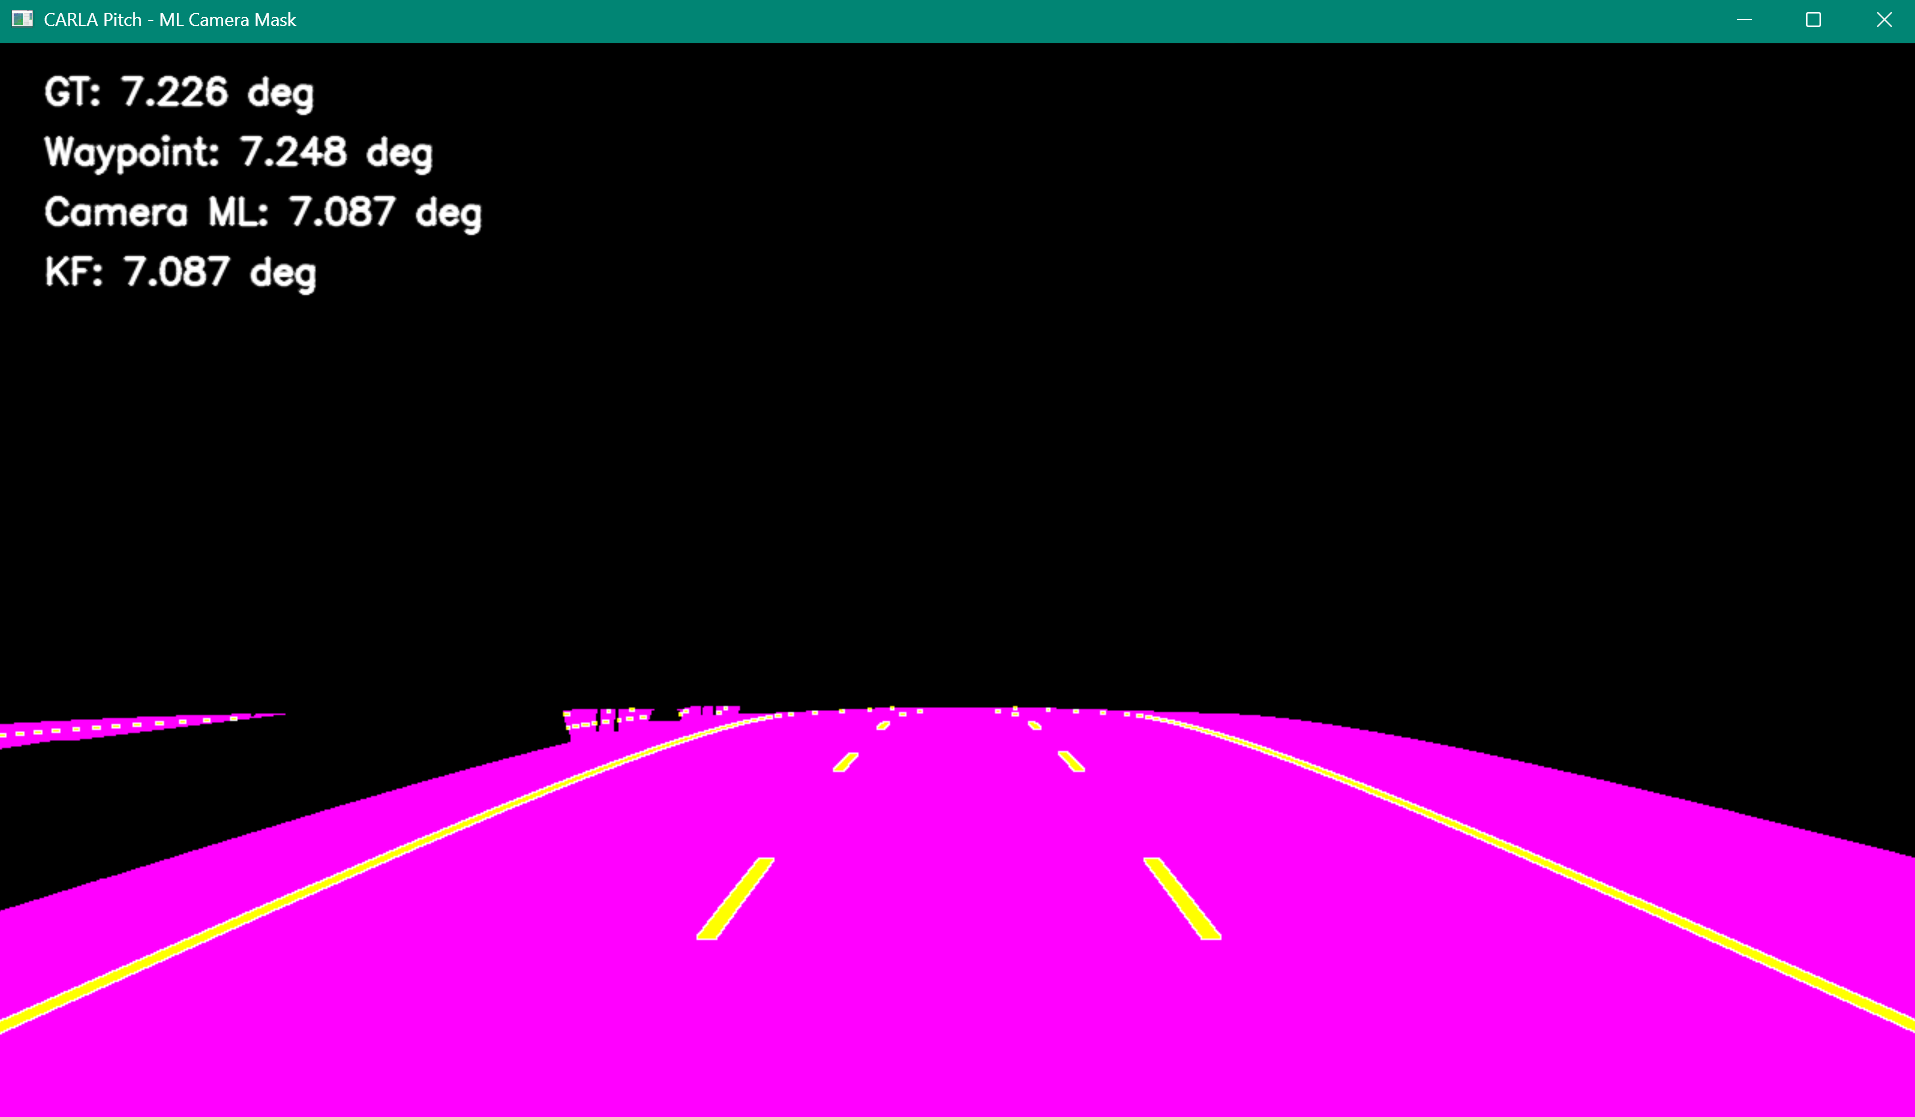
\includegraphics[width=\linewidth]{mask_demo.png}
\column{0.35\textwidth}
\begin{block}{Semantic mask input}
\begin{itemize}
    \item Road pixels are retained
    \item Road-line pixels are retained
    \item Other objects are removed
\end{itemize}
\end{block}
\begin{block}{Why this helps}
The network sees only road geometry, so the pitch regression problem is simplified under controlled CARLA conditions.
\end{block}
\end{columns}
\end{frame}

% ------------------------------------------------------------
\begin{frame}{Final System Overview}
\begin{columns}[T,onlytextwidth]
\column{0.55\textwidth}
\begin{block}{Camera branch}
Semantic Camera $\rightarrow$ Road/Line Mask $\rightarrow$ MobileNetV3 $\rightarrow$ Camera Pitch
\end{block}
\begin{block}{Filter branch}
IMU Gyroscope $\rightarrow$ KF Prediction\\
Camera Pitch $\rightarrow$ KF Correction
\end{block}
\begin{block}{Evaluation branch}
GNSS $\rightarrow$ Baseline Comparison\\
CARLA Truth + Waypoint $\rightarrow$ Reference Signals
\end{block}

\column{0.40\textwidth}
\begin{block}{Key design choice}
The original horizon/vanishing-point camera measurement was replaced with a learned pitch regressor.
\end{block}
\begin{block}{Resulting filter}
Since the camera model directly outputs pitch, the implemented fusion stage becomes a linear Kalman Filter.
\end{block}
\end{columns}
\end{frame}

% ------------------------------------------------------------
\begin{frame}{Tools Used}
\begin{columns}[T,onlytextwidth]
\column{0.48\textwidth}
\begin{block}{Software}
\begin{tabular}{@{}ll@{}}
CARLA & 0.9.16 \\
Python & 3.11 \\
PyTorch & CUDA build \\
CUDA & 13.2 \\
OpenCV & image processing \\
MobileNetV3 & pitch regression \\
\end{tabular}
\end{block}

\column{0.48\textwidth}
\begin{block}{Simulation setup}
\begin{tabular}{@{}ll@{}}
Map & Town05 \\
Vehicle & Tesla Model 3 actor \\
Camera & Semantic segmentation \\
Sampling & 20 Hz \\
Route & ramps + turns \\
GPU & RTX 5070 Ti \\
\end{tabular}
\end{block}
\end{columns}
\smallnote{Full setup instructions and project files are intended to be available in the GitHub repository.}
\end{frame}

% ------------------------------------------------------------
\begin{frame}{Dataset Generation}
\begin{columns}[T,onlytextwidth]
\column{0.44\textwidth}
\begin{block}{Collected data}
\begin{itemize}
    \item Semantic road masks
    \item True vehicle pitch
    \item Waypoint road pitch
    \item IMU and GNSS logs
\end{itemize}
\end{block}
\begin{block}{Split}
Training: 80\%\\
Validation: 20\%
\end{block}

\column{0.52\textwidth}
\begin{block}{Dataset logic}
CARLA drives the selected route automatically. Each camera frame is converted into a road and road-line mask and paired with the corresponding pitch label.
\end{block}
\begin{block}{Training target}
The MobileNet model was trained using true vehicle pitch as the regression target.
\end{block}
\end{columns}
\end{frame}

% ------------------------------------------------------------
\begin{frame}{MobileNet Training Results}
\begin{columns}[T,onlytextwidth]
\column{0.49\textwidth}
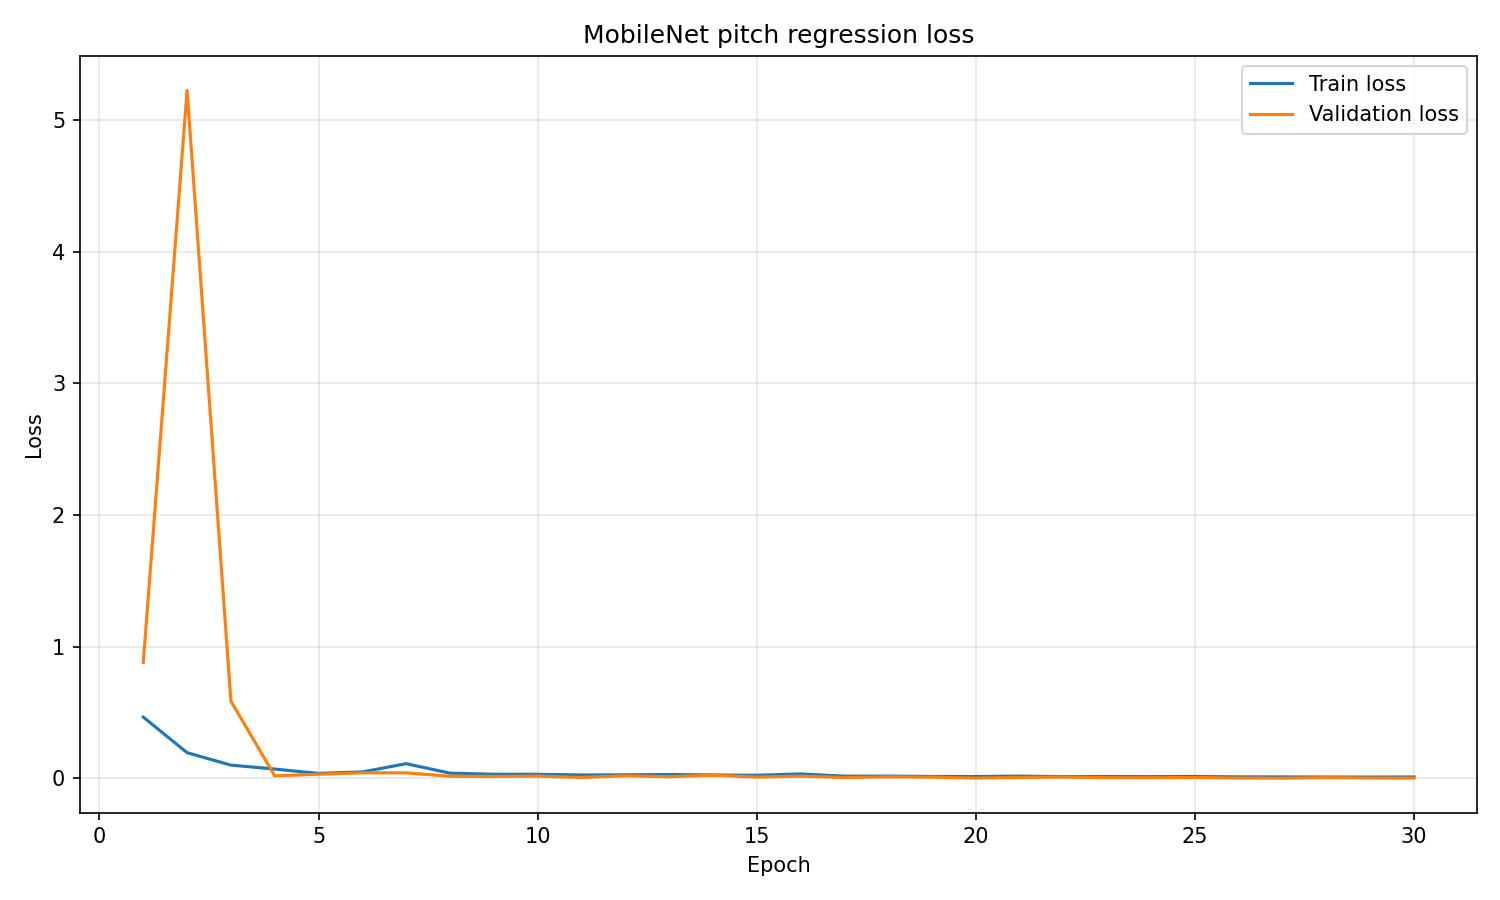
\includegraphics[width=\linewidth]{loss_curve.png}
\column{0.49\textwidth}
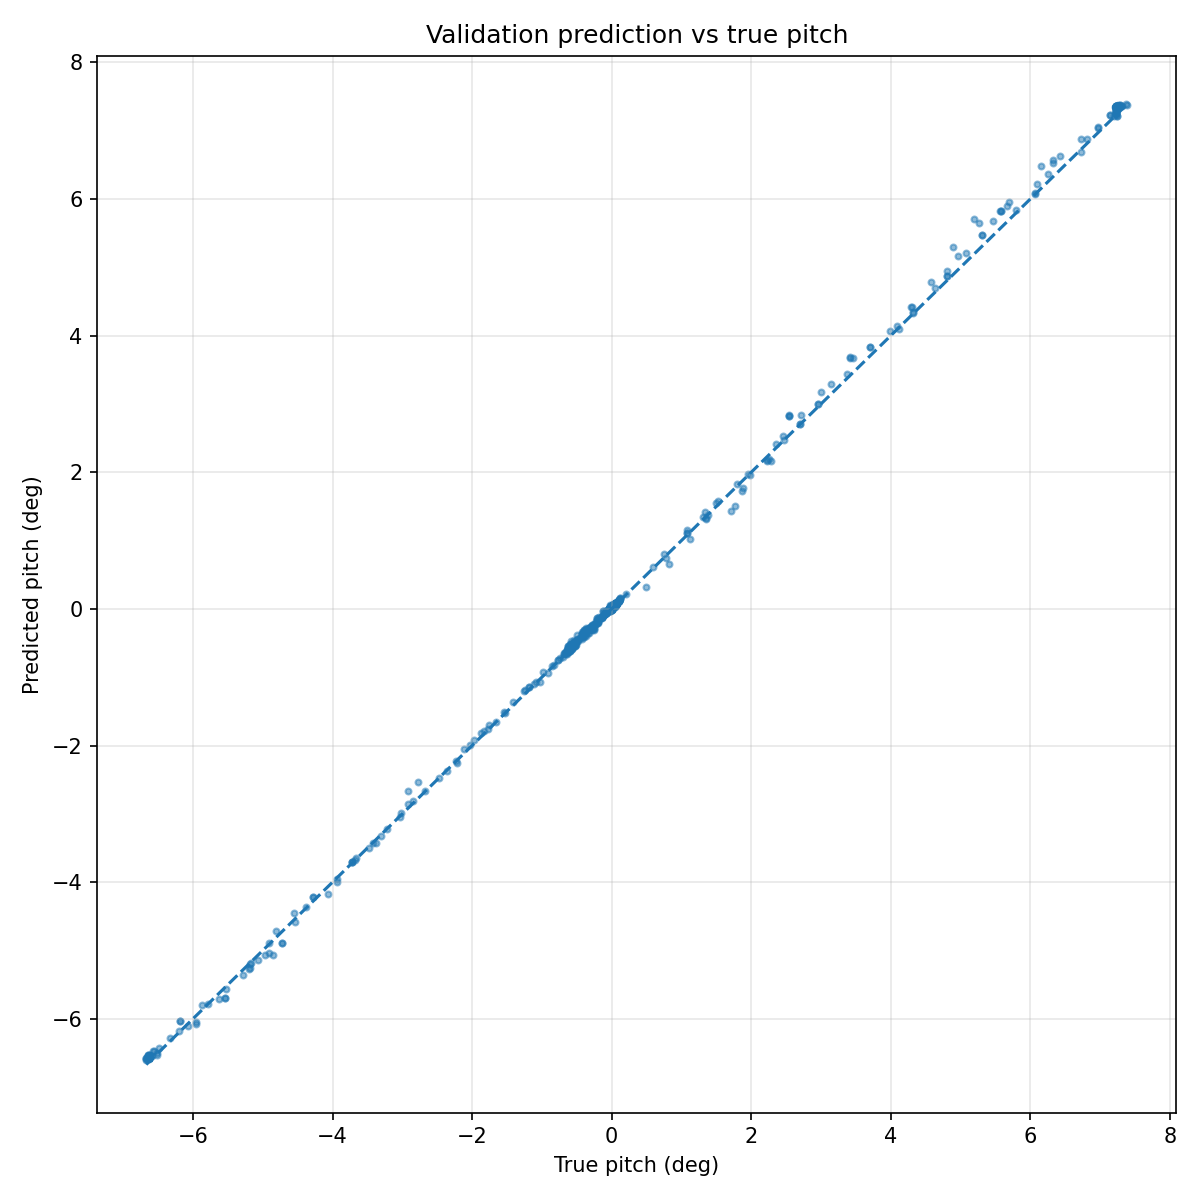
\includegraphics[width=\linewidth]{val_scatter.png}
\end{columns}
\smallnote{The validation prediction plot shows that the model learned the pitch range in the collected CARLA dataset.}
\end{frame}

% ------------------------------------------------------------
\begin{frame}{Kalman Filter: Prediction Step}

\begin{block}{IMU-Based Pitch Propagation}

The IMU gyroscope provides pitch rate measurements.

\[
\hat{\theta}_k^{-}
=
\hat{\theta}_{k-1}
+
\omega_{y,k}\Delta t
\]

\end{block}

\vspace{0.3cm}

\begin{block}{Uncertainty Prediction}

The uncertainty grows during prediction:

\[
P_k^{-}
=
P_{k-1}
+
Q
\]

\end{block}

\end{frame}

\begin{frame}{Kalman Filter: Camera Correction}

\begin{block}{Camera Measurement}

The MobileNet model produces a pitch estimate:

\[
z_k
=
\theta_{camera}
\]

\end{block}

\vspace{0.3cm}

\begin{block}{Kalman Gain}

\[
K_k
=
\frac{P_k^{-}}
     {P_k^{-}+R}
\]

\end{block}

\vspace{0.3cm}

\begin{block}{State Correction}

\[
\hat{\theta}_k
=
\hat{\theta}_k^{-}
+
K_k
\left(
z_k-\hat{\theta}_k^{-}
\right)
\]

\end{block}



\small
The camera estimate corrects accumulated IMU drift and improves long-term stability.

\end{frame}

\begin{frame}{Kalman Filter: Parameters}
\begin{block}{Parameters}

\[
\omega_{y,k}
=
\text{IMU gyroscope pitch rate}
\]
\[
Q = 0.01
\]
\[R = 0.01\]

\end{block}

\small
The IMU provides short-term pitch propagation between camera measurements.

\end{frame}
% ------------------------------------------------------------
\begin{frame}{Camera and GNSS Results}
\begin{columns}[T,onlytextwidth]
\column{0.49\textwidth}
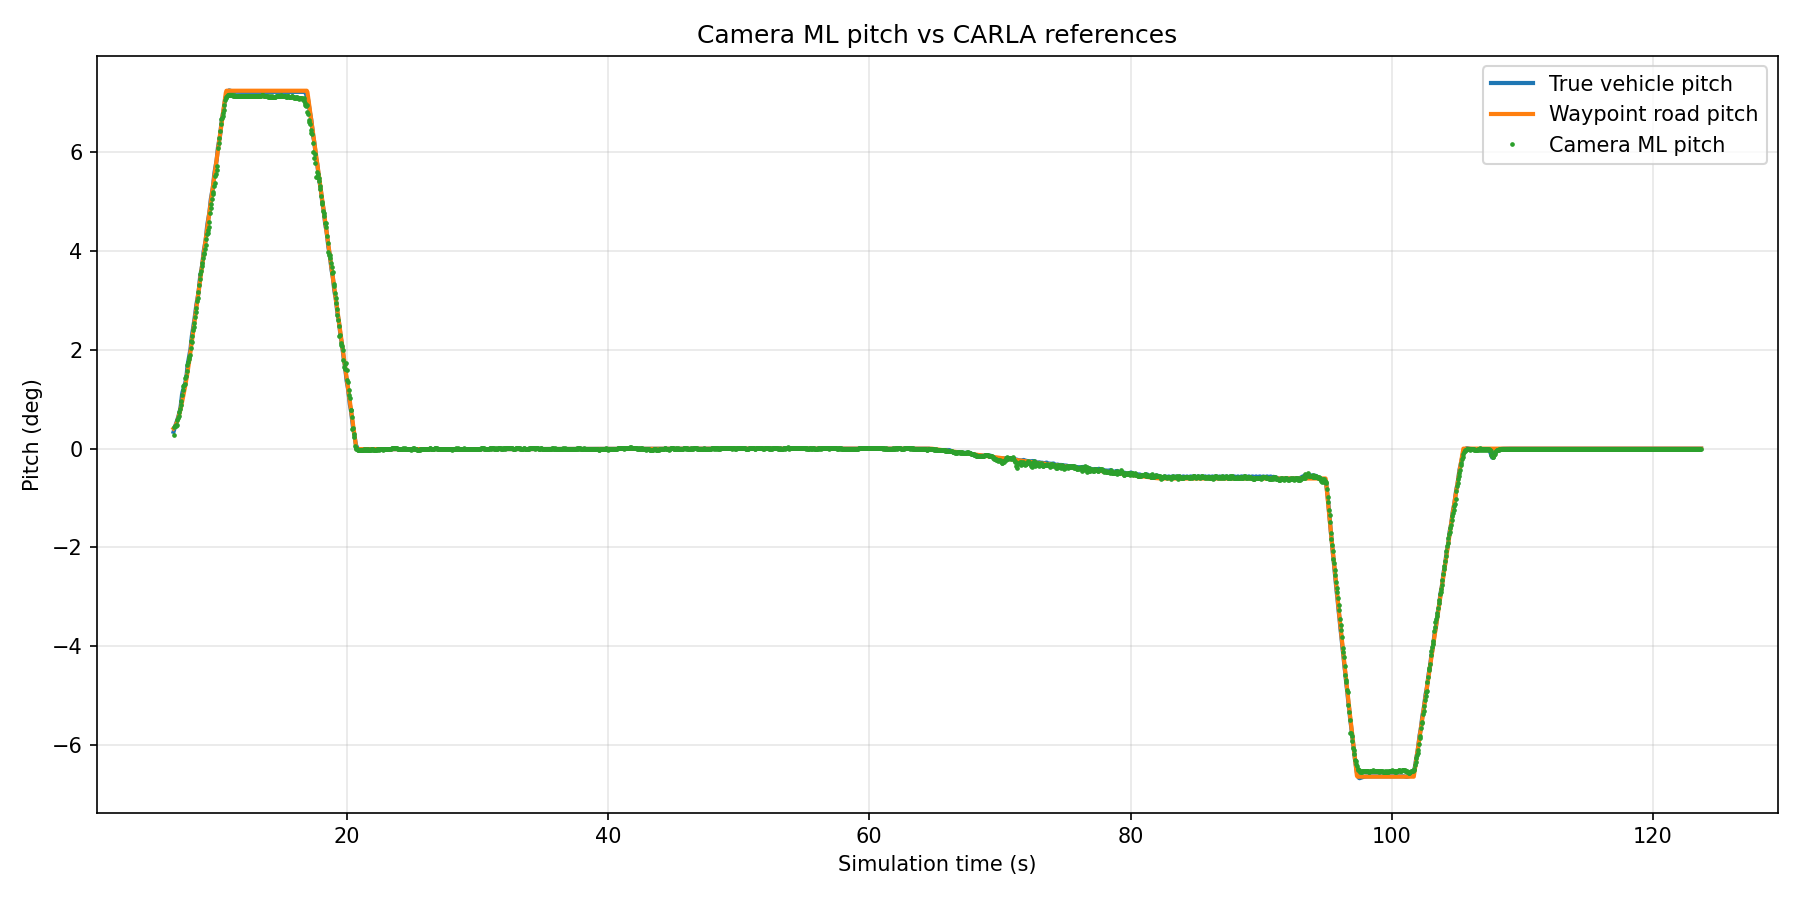
\includegraphics[width=\linewidth]{camera_pitch.png}
\column{0.49\textwidth}
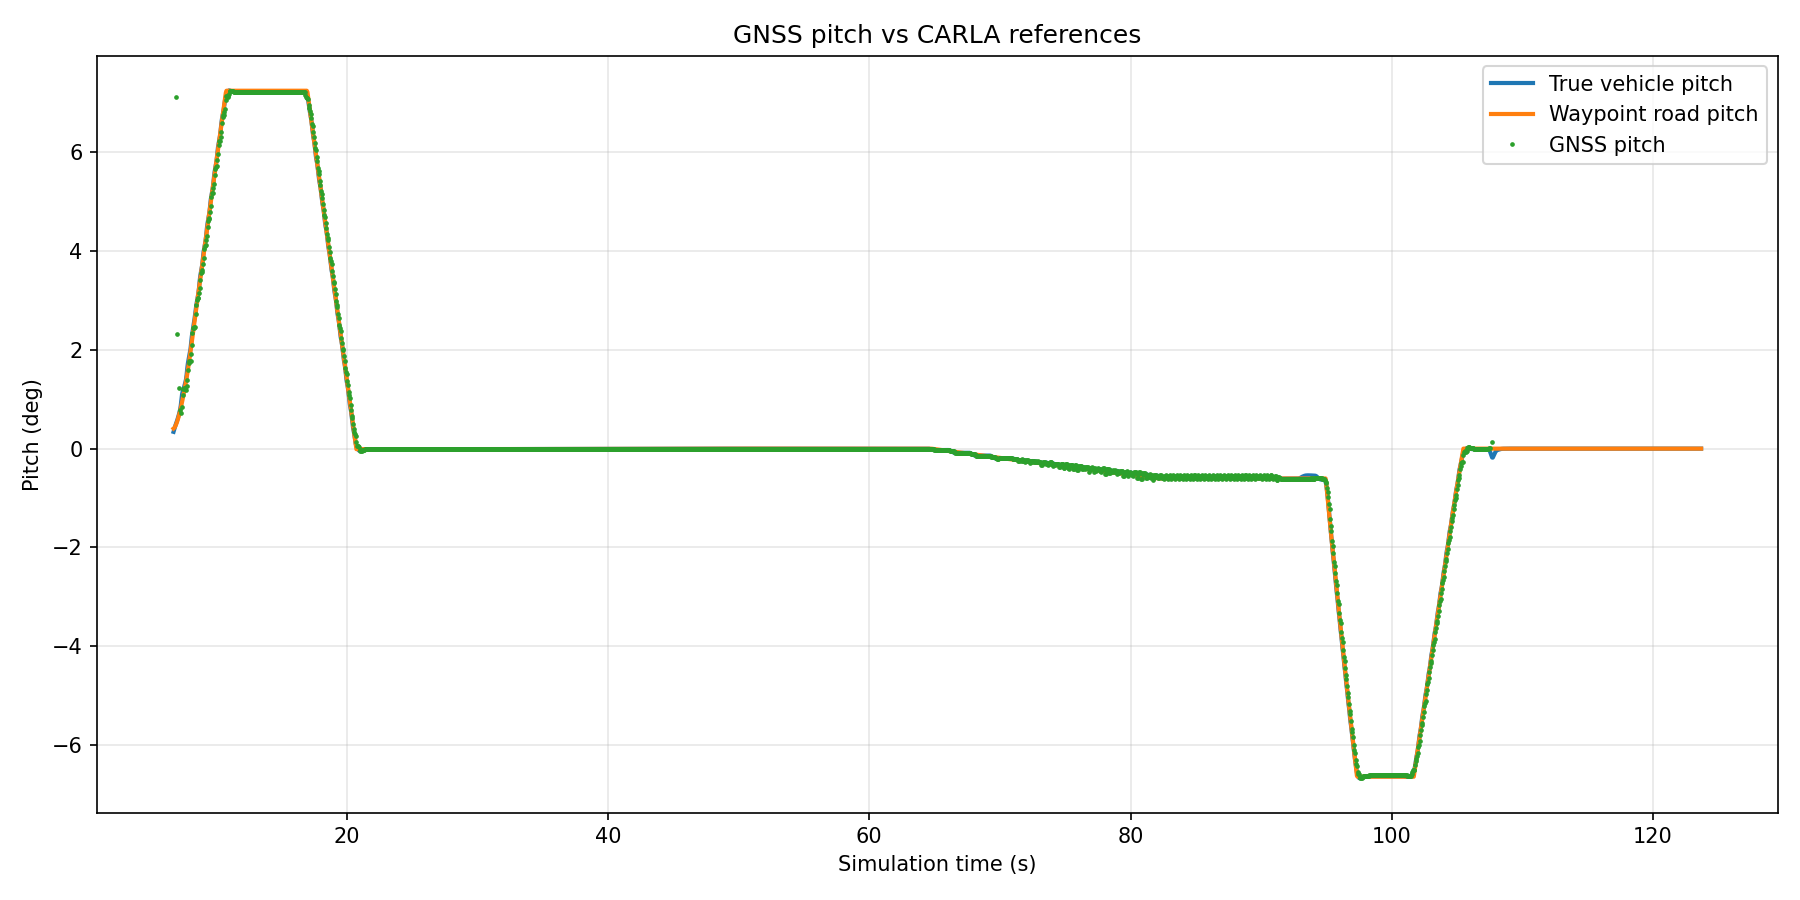
\includegraphics[width=\linewidth]{gnss_pitch.png}
\end{columns}
\smallnote{GNSS pitch is useful as a baseline, but it depends on horizontal displacement and can become unavailable during stops.}
\end{frame}

% ------------------------------------------------------------
\begin{frame}{Combined Results}
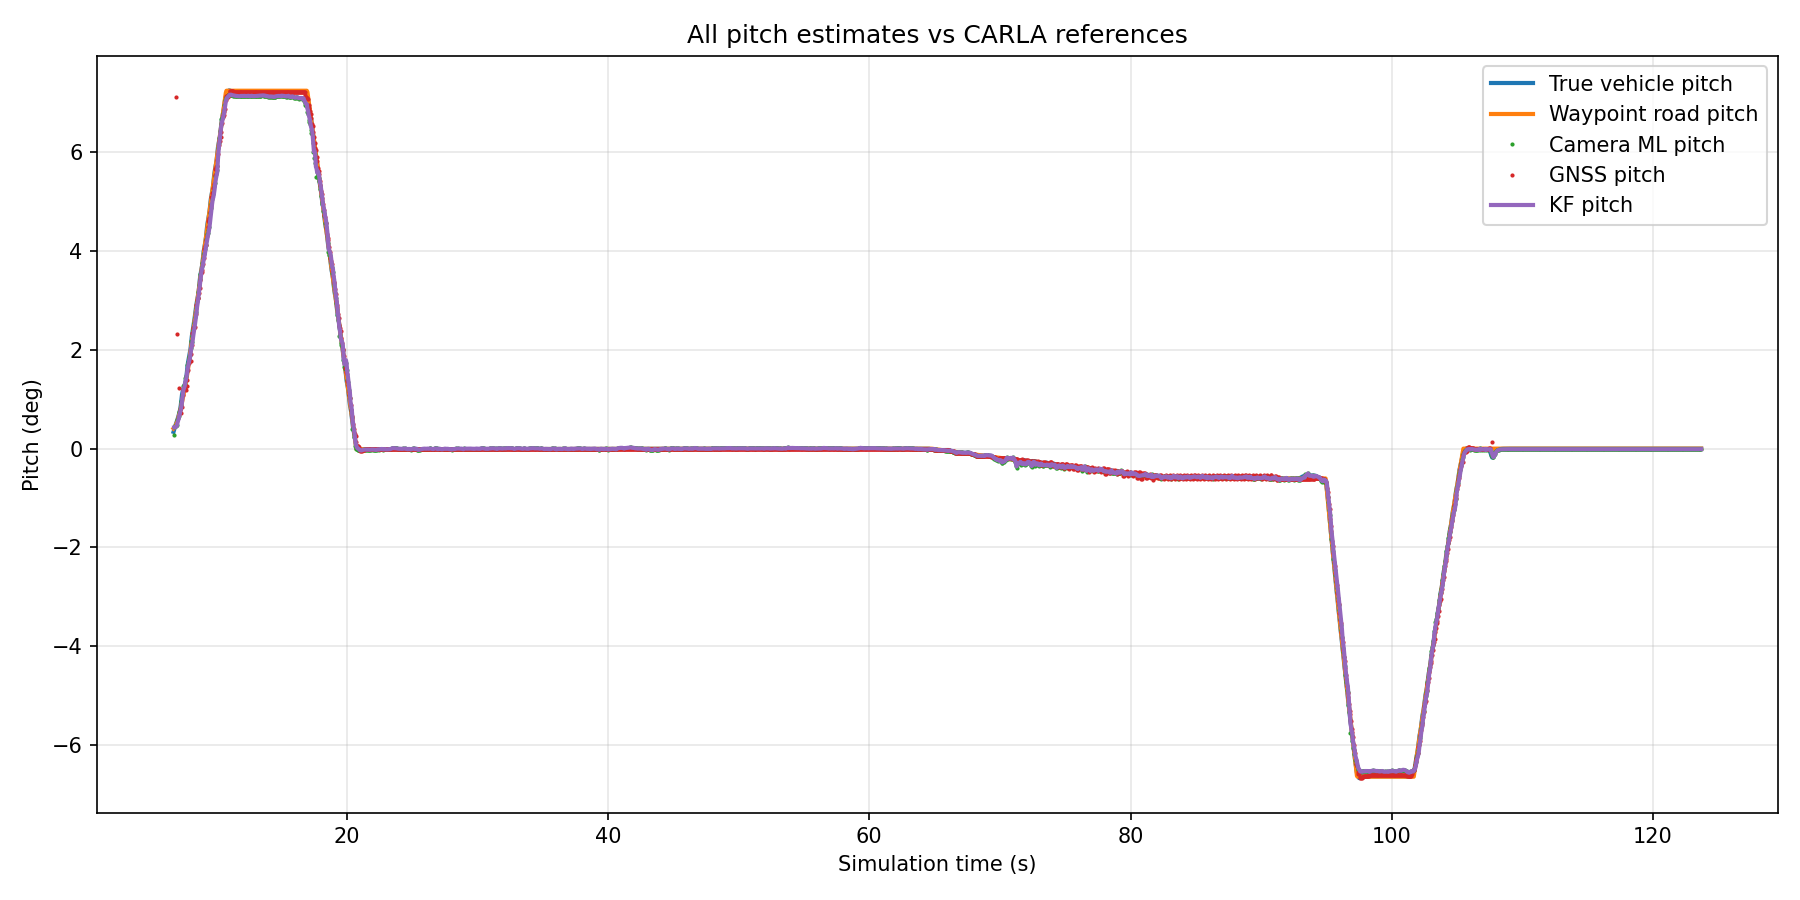
\includegraphics[width=\linewidth,height=0.76\textheight,keepaspectratio]{all_sensors.png}
\smallnote{Camera and KF remain available at each camera frame. GNSS is only evaluated when displacement is sufficient.}
\end{frame}

% ------------------------------------------------------------
\begin{frame}{Quantitative Error Summary}
\centering
\begin{tabular}{lccc}
\toprule
Estimate & MAE (deg) & RMSE (deg) & Max (deg) \\
\midrule
Camera vs true     & 0.028 & 0.050 & 0.408 \\
Camera vs waypoint & 0.032 & 0.057 & 0.465 \\
GNSS vs true       & 0.023 & 0.158 & 6.611 \\
GNSS vs waypoint   & 0.024 & 0.158 & 6.632 \\
KF vs true         & 0.034 & 0.063 & 0.366 \\
KF vs waypoint     & 0.035 & 0.062 & 0.349 \\
\bottomrule
\end{tabular}
\vspace{1em}
\begin{block}{Interpretation}
The camera model is highly accurate in this controlled CARLA route. In less controlled conditions, IMU-assisted filtering is expected to become more useful when camera measurements degrade or disappear.
\end{block}
\end{frame}

% ------------------------------------------------------------
\begin{frame}{Code Structure}
\begin{columns}[T,onlytextwidth]
\column{0.48\textwidth}
\begin{block}{Main scripts}
\begin{tabular}{@{}ll@{}}
01 & collect pitch dataset \\
02 & train MobileNet model \\
05 & run KF evaluation \\
\end{tabular}
\end{block}
\begin{block}{Outputs}
CSV logs, error summary, trained model, plots, mask images.
\end{block}

\column{0.48\textwidth}
\begin{block}{Run order}
\begin{enumerate}
    \item Start CARLA 0.9.16
    \item Collect dataset
    \item Train model
    \item Run final KF script
    \item Export plots and metrics
\end{enumerate}
\end{block}
\end{columns}
\end{frame}

% ------------------------------------------------------------
\begin{frame}{Setup and Running}
\begin{block}{Requirements}
CARLA 0.9.16, Python 3.11, PyTorch CUDA build, OpenCV, torchvision, matplotlib.
\end{block}

\begin{block}{Typical workflow}
\begin{enumerate}
    \item Download and run CARLA 0.9.16.
    \item Create a Python 3.11 virtual environment.
    \item Install dependencies listed in the GitHub repository.
    \item Run dataset collection, training, and final evaluation scripts.
\end{enumerate}
\end{block}

\smallnote{The public GitHub repository should contain exact commands, project structure, example outputs, and the final paper PDF.}
\end{frame}

% ------------------------------------------------------------
\begin{frame}{Limitations and Conclusion}
\begin{columns}[T,onlytextwidth]
\column{0.48\textwidth}
\begin{block}{Limitations}
\begin{itemize}
    \item Controlled CARLA route
    \item Semantic masks instead of real RGB camera input
    \item Limited road/environment variety
    \item No real-world sensor validation yet
\end{itemize}
\end{block}

\column{0.48\textwidth}
\begin{block}{Conclusion}
\begin{itemize}
    \item CARLA pitch dataset generated
    \item MobileNet pitch regressor trained
    \item GNSS baseline evaluated
    \item IMU-camera KF implemented
    \item Results match CARLA references closely
\end{itemize}
\end{block}
\end{columns}
\vspace{0.5em}
\centering
\textbf{Repository and paper links will be provided in the video description.}
\end{frame}

% ------------------------------------------------------------
\begin{frame}{Sources and Thank You}

\scriptsize

\textbf{Main References}

\vspace{0.3cm}

Key sources cover monocular road estimation \cite{ustunel2023iterative}, the CARLA simulator \cite{dosovitskiy2017carla}, MobileNetV3 \cite{howard2019mobilenetv3}, and PyTorch \cite{paszke2019pytorch}.

\vspace{0.2cm}

\bibliographystyle{IEEEtran}
\bibliography{refs}

\vfill

\centering
{\Large Thank You for Watching}


\end{frame}

\end{document}
